\documentclass[11pt, a4paper, twoside]{article}   	% use "amsart" instead of "article" for AMSLaTeX format

\usepackage{geometry}                		% See geometry.pdf to learn the layout options. There are lots.
\usepackage{pdfpages}
\usepackage{caption}
\usepackage{minted}
\usepackage[german]{babel}			% this end the next are needed for german umlaute
\usepackage[utf8]{inputenc}
\usepackage{color}
\usepackage{graphicx}
\usepackage{titlesec}
\usepackage{fancyhdr}
\usepackage{lastpage}
\usepackage{hyperref}
% http://www.artofproblemsolving.com/wiki/index.php/LaTeX:Symbols#Operators
% =============================================
% Layout & Colors
% =============================================
\geometry{
   a4paper,
   total={210mm,297mm},
   left=20mm,
   right=20mm,
   top=20mm,
   bottom=30mm
 }	

\definecolor{myred}{rgb}{0.8,0,0}
\definecolor{mygreen}{rgb}{0,0.6,0}
\definecolor{mygray}{rgb}{0.5,0.5,0.5}
\definecolor{mymauve}{rgb}{0.58,0,0.82}

\setcounter{secnumdepth}{4}


% the default java directory structure and the main packages
\newcommand{\srcDir}{/src/main/java}
% =============================================
% Code Settings
% =============================================
\newenvironment{code}{\captionsetup{type=listing}}{}
\newmintedfile[javaSourceFile]{java}{
	linenos=true, 
	frame=single, 
	breaklines=true, 
	tabsize=2,
	numbersep=5pt,
	xleftmargin=10pt,
	baselinestretch=1,
	fontsize=\footnotesize
}
\newmintinline[inlineJava]{java}{}
\newminted[javaSource]{java}{
	breaklines=true, 
	tabsize=2,
	autogobble=true,
	breakautoindent=false
}
\newmintedfile[xmlSourceFile]{xml}{
	linenos=true, 
	frame=single, 
	breaklines=true, 
	tabsize=2,
	numbersep=5pt,
	xleftmargin=10pt,
	baselinestretch=1,
	fontsize=\footnotesize
}
\newmintedfile[propertiesFile]{properties}{
	linenos=true, 
	frame=single, 
	breaklines=true, 
	tabsize=2,
	numbersep=5pt,
	xleftmargin=10pt,
	baselinestretch=1,
	fontsize=\footnotesize
}
\newmintedfile[sqlFile]{sql}{
	linenos=true, 
	frame=single, 
	breaklines=true, 
	tabsize=2,
	numbersep=5pt,
	xleftmargin=10pt,
	baselinestretch=1,
	fontsize=\footnotesize
}
% =============================================
% Page Style, Footers & Headers, Title
% =============================================
\title{Übung 3}
\author{Thomas Herzog}

\lhead{Übung 3}
\chead{}
\rhead{
\includegraphics[scale=0.10]{FHO_Logo_Students.jpg}}

\lfoot{S1310307011}
\cfoot{}
\rfoot{ \thepage / \pageref{LastPage} }
\renewcommand{\footrulewidth}{0.4pt}
% =============================================
% D O C U M E N T     C O N T E N T
% =============================================
\pagestyle{fancy}
\begin{document}
\setlength{\headheight}{15mm}
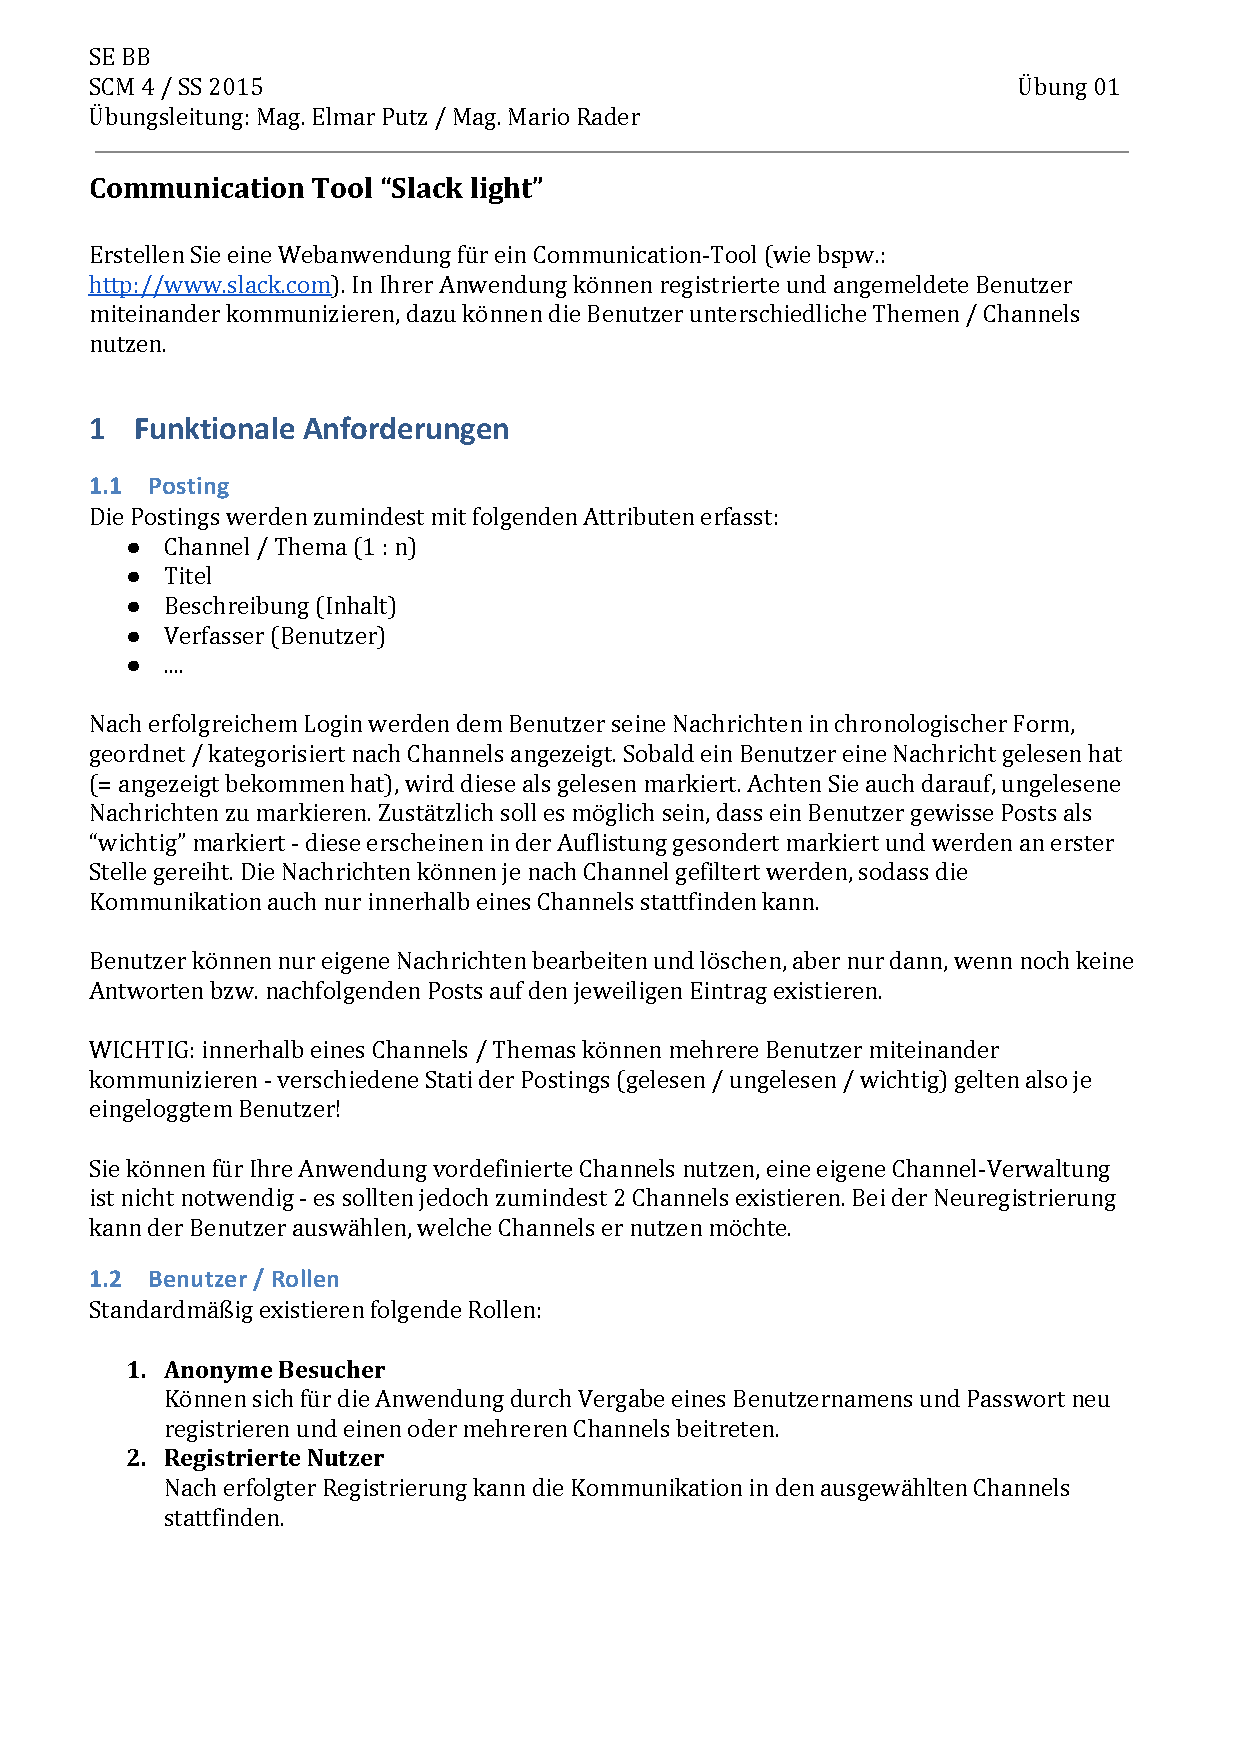
\includepdf[pages={1,2,3}]{scm4-2015-uebung01-communication-list.pdf}
{\color{myred}
	\section
		{Kommunikationstool 'Slack Light'}
}

\subsection{Setup}
Für das Aufsetzten wird lediglich das Anlegen der Datenbank benötigt, welches die Datenbank anlegt, einen Benutzer sowie zwei vordefinierte Channels erstellt.\\
Das Skript ist verfügbar unter \textbf{PROJECT\textbackslash internal\textbackslash db\textbackslash create.sql}\\\\
Die Datenbankkonfiguration seitens PHP ist in\\
\textbf{PROJECT\textbackslash source\textbackslash db\textbackslash controller\textbackslash AbstractEntityController.php}\\
enthalten.\\\\
\textbf {Username:} 'het'\\
\textbf {Password:} '123'\\\\
\newpage 

\subsection{Datenbank}
Folgende Abbildung zeigt das ER Diagramm des Datenmodells für das Kommunikationstool "Slack light". \
\begin{figure}[h]
	\centering
	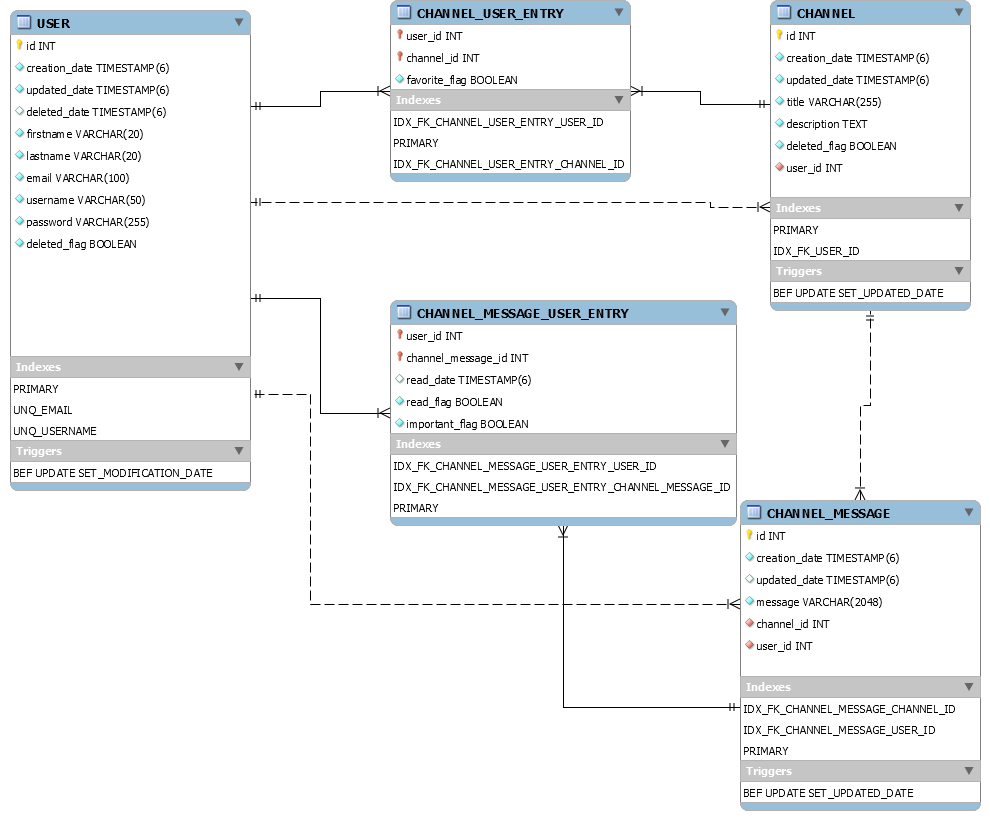
\includegraphics[scale=0.5]{images/er-model.PNG}
	\caption
	{ER-Modell}
\end{figure}

\newpage
\subsection{Applikationsarchitektur}
Folgender Abschnitt beschreibt die Architektur der Applikation.\\
Die Applikation ist in zwei Haupt PHP Dateien aufgeteilt über die alle Requests abgearbeitet werden:
\begin{enumerate}
	\item \textbf{index.php:} \\
	All offenen Ressourcen wie Login und Registrierung (Kein Login erforderlich)
	\item \textbf{start.php:} \\
	Alle geschützten Ressourcen. (Login erforderlich).
\end{enumerate}
Diese beiden *.php Dateien Dateien sowie alle *.css, *.js Dateien und Images sind in einem öffentlichen Verzeichnis (public) zusammengefasst und können ohne Zugriffskontrolle abgerufen werden. (Kein eingeloggter Benutzer erforderlich)\\
Alle anderen angezeigten Seiten werden über das Templating Tool \textbf{Twig} generiert und werden über die beiden PHP Dateien index.php oder start.php and den Client übermittelt. Dadurch ist kein direkter Zugriff auf diese Dateien möglich.
\\\\
Folgende Abbildung illustriert die Architektur der Applikation beziehungsweise den Ablauf eines Requests. \\
\begin{figure}[h]
	\centering
	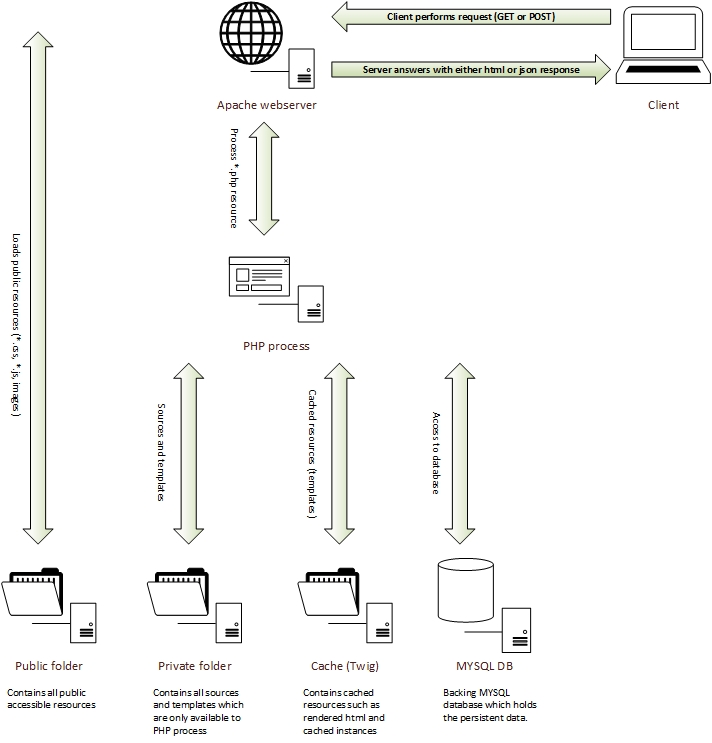
\includegraphics[scale=0.70]{images/Infrastructure.JPG}
	\caption
	{Applikationsarchitektur}
\end{figure}

\newpage 
Die Applikation wurde in 3 Ebenen unterteilt, wobei nicht alle Ebenen nach außen frei zugänglich sind.\\
\begin{enumerate}
	\item \textbf{public/*} \\
	Enthält alle öffentlich und ohne Einschränkung zugängliche Ressourcen. Diese Ressourcen sind direkt über den Webserver zugänglich und müssen nicht von einem PHP Prozess bearbeitet werden. Diese sind z.B.: Javascript-, CSS- und Image-Dateien. Die beiden Hauptseiten index.php und start.php stellen hierbei eine Ausnahme dar. Sie werden zwar von einem PHP Prozess abgearbeitet werden aber nicht von einem PHP Prozess generiert.  
	\item \textbf{source/*} \\
	Alle geschützten Ressourcen wie die PHP Sources und die Twig Templates. Sie sind nur über den PHP Prozess und Source in index.php und start.php erreichbar. Dadurch sind die Sources von außen abgeschirmt, wobei der Webserver diese Verzeichnisse von einem externen zugriff zu schützen hat.
	\item \textbf{cache/*}\\
	Enthält die kompilierten Twig Templates sowie die erstellten Html-Dateien, somit müssen diese nicht bei jeder Verarbeitung neu kompiliert oder erstellt werden. Der Code entschiedet hierbei ob ein erneutes Erstellen erforderlich ist oder nicht.
\end{enumerate}
Es werden zwei externe Libraries verwendet, die zwar über Composer geladen wurden aber über einen eigenen Autoloader innerhalb des PHP Prozess geladen werden.
\begin{enumerate}
	\item \textbf{Twig:}\\
	Hierbei handelt es sich um eine Template Library, die dazu verwendet wird um die Html-Dateien für den Client aufzubereiten. Hierzu wird ein Assoziativen Array mit Parametern befüllt, welche innerhalb der Twig-Template-Engine verarbeiten werden um das zu übermittelnde Html zu produzieren. Dabei ist kein PHP Source in den Html-Dateien enthalten, was meiner Meinung nach die Übersichtlichkeit erhöht. Der dynamische Inhalt wird innerhalb des PHP Codes aufbereitet und nur die Ausgabeparameter an die Twig-Template-Engine weitergereicht.
	\item \textbf{Stash:}\\
	Hierbei handelt es sich um eine Caching Library, welche dazu verwendet wird um die erstellten Html-Dateien zu speichern, damit diese nicht immer neu verarbeitet werden müssen. Im PHP Code wird entschieden ob eine Html-Datei neu erstellt werden soll oder ob diese aus den Cache genommen werden soll.
\end{enumerate}
\newpage

\subsection{Tests}
Folgend sind die Tests für die Applikation angeführt.
\subsubsection{Benutzerregistrierung}
Folgend sind die Tests für die Benutzerregistrierung angeführt.\\\\
Folgender Test zeigt die angewendete Client Validierung über Bootstrap-Form-Validation Plugin. 
\begin{figure}[h]
	\centering
	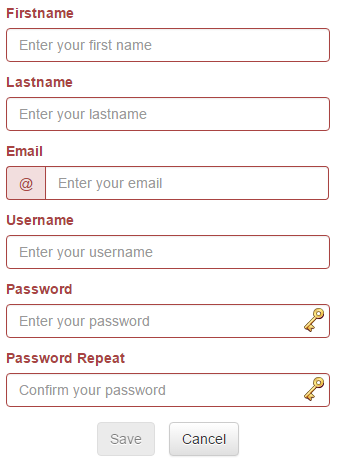
\includegraphics[scale=0.5]{images/registration_client_validation_full.PNG}
	\caption
	{Bootstrap Form Validation}
\end{figure}\\\\
Neben der Required Validerung erfolgt auch eine Validierung auf eine syntaktisch gültige E-Mail Adresse.
\begin{figure}[h]
	\centering
	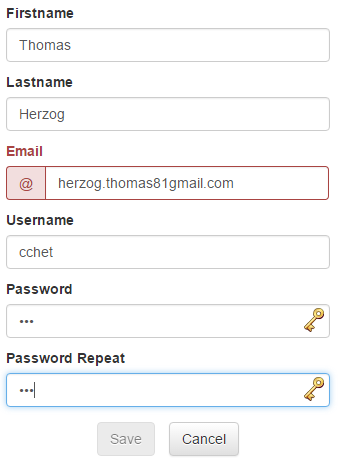
\includegraphics[scale=0.5]{images/registration_client_validation_email.PNG}
	\caption
	{Bootstrap Form Validation E-Mail}
\end{figure}
\newpage
Wenn eine E-Mail bereits von einem Benutzer verwendet wird, dann wird dies serverseitig Validiert und an eine Fehlermeldung an den Client übermittelt.
\begin{figure}[h]
	\centering
	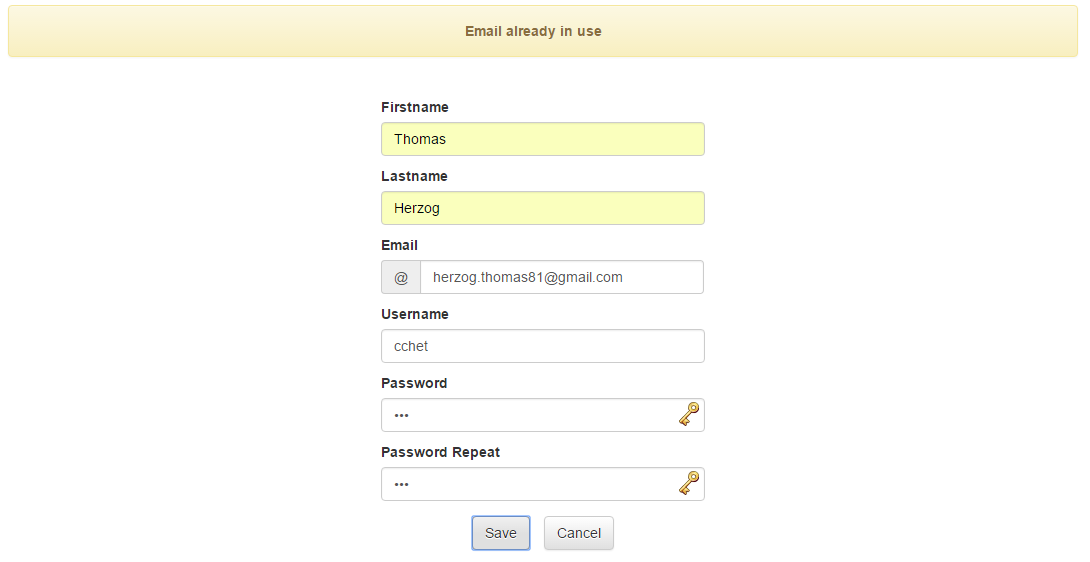
\includegraphics[scale=0.4]{images/registration_server_validation_email.PNG}
	\caption
	{Serverseitige E-Mail Validierung}
\end{figure}\\\\
Wenn ein Benutzername bereits von einem aktiven Benutzer verwendet wird, dann wird dies serversetig validiert und eine Fehlermeldung and den Client übermittelt.
\begin{figure}[h]
	\centering
	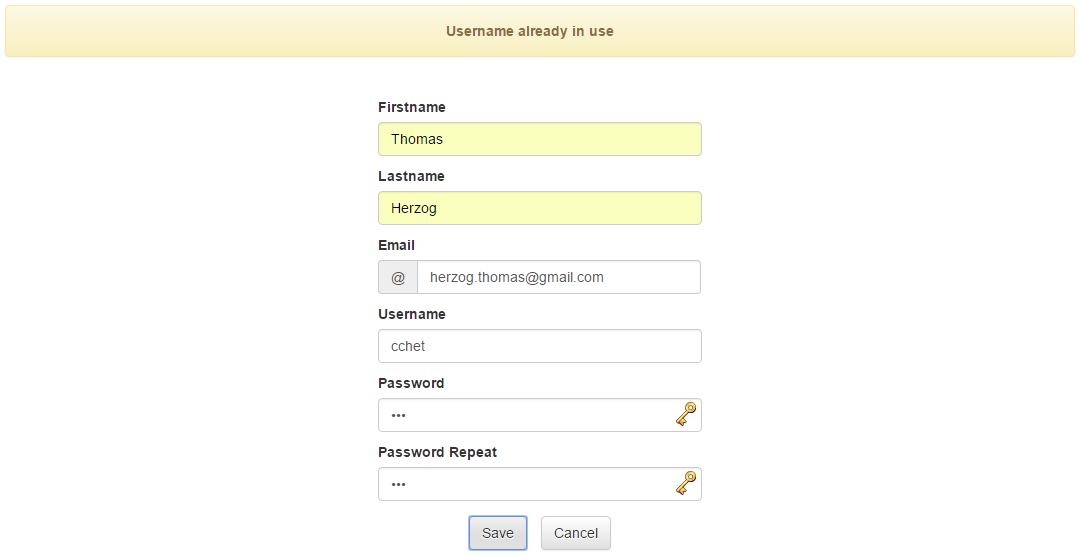
\includegraphics[scale=0.4]{images/registration_server_validation_username.PNG}
	\caption
	{Serverseitige Benutzernamen Validierung}
\end{figure}
\newpage
Nach der erfolgreichen Registrierung eines Benutzers wird eine Erfolgsmeldung angezeigt, wobei nach einigen Sekunden automatisch auf die Login Seite weitergeleitet wird, obwohl ebenfalls eine Button zur Verfügung steht, der auf die Login Seite wechselt sollte das automatische Weiterleiten nicht funktionieren.
\begin{figure}[h]
	\centering
	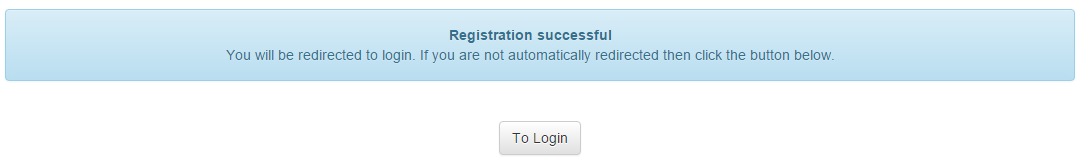
\includegraphics[scale=0.6]{images/registration_success.PNG}
	\caption
	{Registrierung erfolgreich}
\end{figure}\\\\
\newpage

\subsubsection{Login}
Folgend sind die Tests für den Login angeführt.\\\\
Folgender Test zeigt die angewendete Client Validierung über Bootstrap-Form-Validation Plugin. 
\begin{figure}[h]
	\centering
	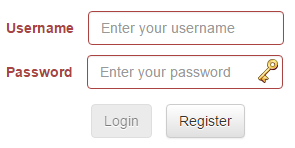
\includegraphics[scale=0.5]{images/login_client_validation_full.PNG}
	\caption
	{Bootstrap Form Validation}
\end{figure}\\\\
Folgender Test zeigt die serversetige Validierung der Login Daten.
\begin{figure}[h]
	\centering
	
\includegraphics[scale=0.5]{images/login_server_validation_credentials.PNG}
	\caption
	{Serverseitige Validierung Login Daten (Benutzername, Passwort)}
\end{figure}\\\\

\newpage

\subsubsection{Channel Verwaltung}
Folgend sind die Tests für die Channel Verwaltung angeführt, die nur eingeloggte Benutzer sehen können und nur Benutzer, die die Channels angelegt haben dürfen diese auch bearbeiten.\\
Sollten Channels gelöscht werden alle abhängigen Daten ebenso gelöscht (Benutzereinträge, Nachrichten).\\\\
Folgender Test zeigt dass wenn es noch keine Channels gibt, der Benutzer immer die Seite für das Anlegen eines Channels angezeigt bekommt. Diese Seite bekommt er solange angezeigt bis mindestens ein Channel existiert, egal welchen Link (außer Logout) er anklickt. Eine entsprechende Meldung wird ebenso angezeigt.
\begin{figure}[h]
	\centering
	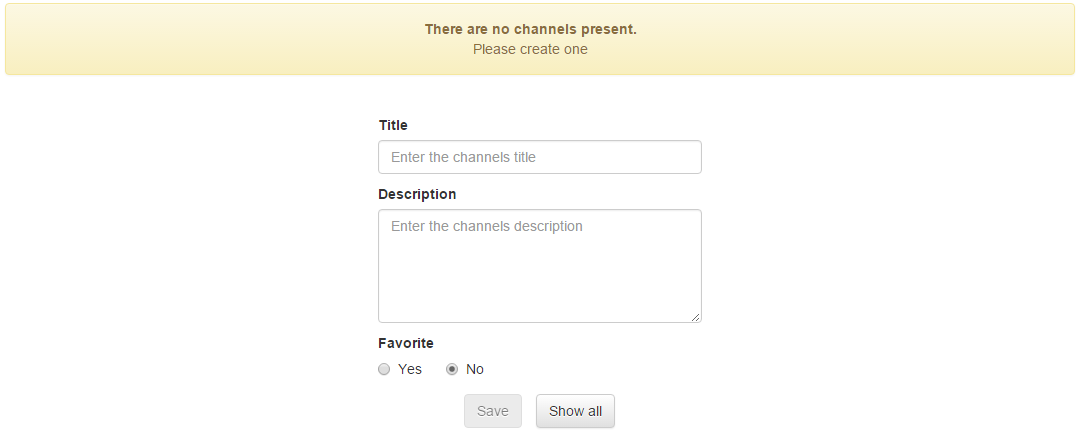
\includegraphics[scale=0.5]{images/start_new_channel_no_channels.PNG}
	\caption
	{Channel anlegen wenn keine vorhanden}
\end{figure}\\\\

Folgender Test zeigt die Erfolgsmeldung wenn ein Channel von einem Benutzer angelegt wurde.
\begin{figure}[h]
	\centering
	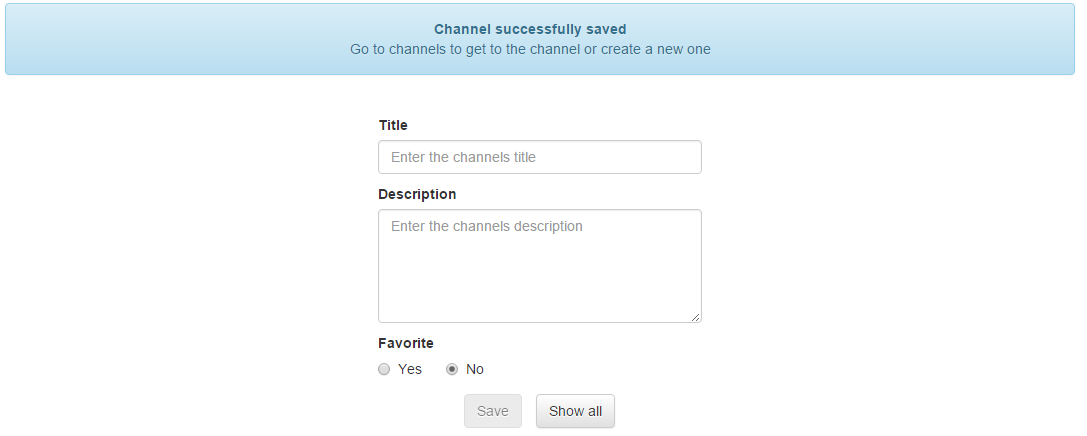
\includegraphics[scale=0.5]{images/start_new_channel_successful.PNG}
	\caption
	{Channel erfolgreich angelegt}
\end{figure}\\\\
\newpage

Folgender Test zeigt die Fehlermeldung wenn ein Channel von einem Benutzer versucht wird anzulegen dieser aber bereits mit dem eingegebenen Titel existiert. Groß- und Kleinschreibung wird hier ignoriert.
\begin{figure}[h]
	\centering
	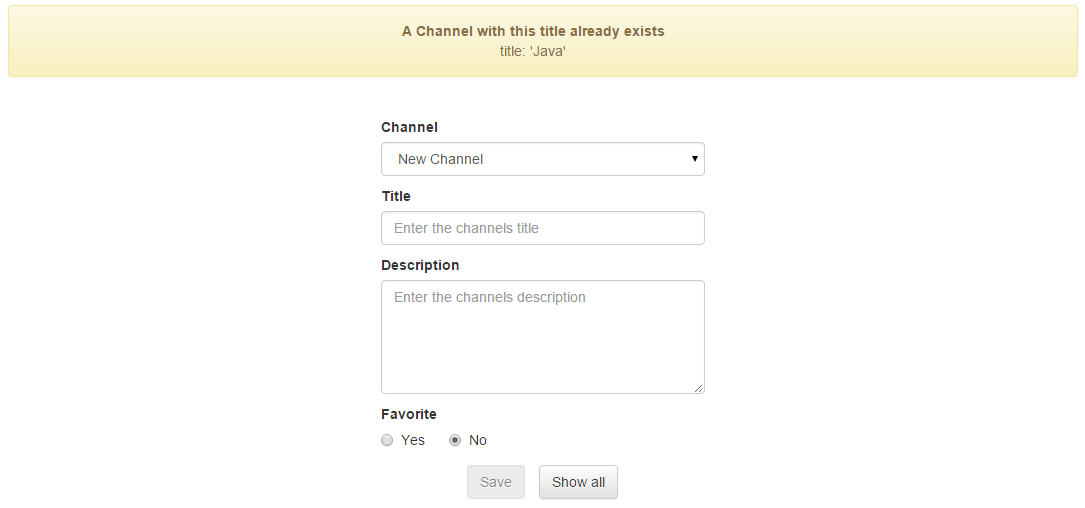
\includegraphics[scale=0.5]{images/start_new_channel_already_existing.PNG}
	\caption
	{Channel existiert bereits}
\end{figure}\\\\

Folgender Test zeigt die Fehlermeldung wenn versucht wird einen Channel zu selektieren/updaten/löschen und dieser nicht mehr existiert.
\begin{figure}[h]
	\centering
	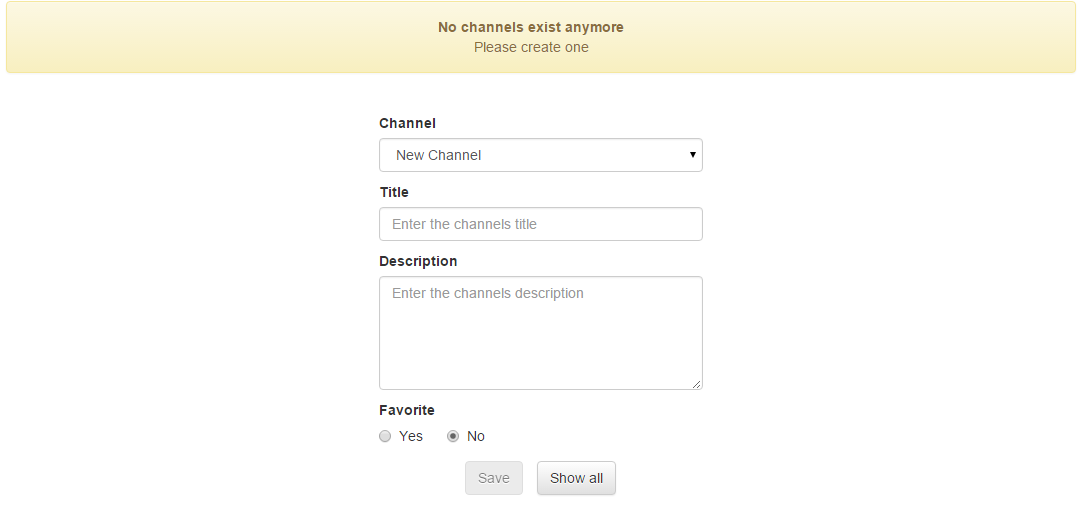
\includegraphics[scale=0.5]{images/start_new_channel_already_deleted.PNG}
	\caption
	{Channel existiert bereits}
\end{figure}\\\\
\newpage

Folgender Test zeigt die Fehlermeldung wenn ein Channel versucht wird upzudaten, der Benutzer aber keine Änderungen angegeben hat.
\begin{figure}[h]
	\centering
	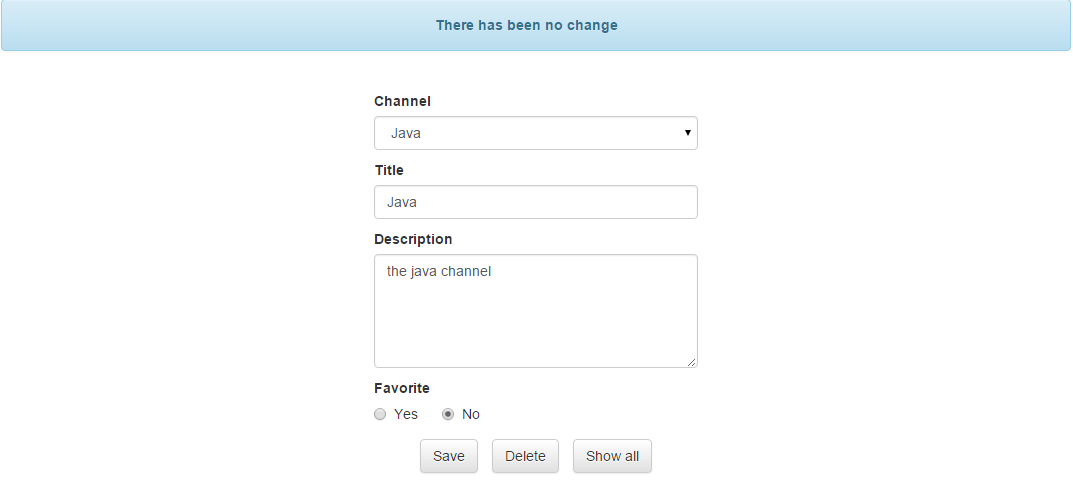
\includegraphics[scale=0.5]{images/start_new_channel_no_change.PNG}
	\caption
	{Channel existiert bereits}
\end{figure}\\\\

Folgender Test zeigt die implizite Zuweisung eines Channels zu dem Benutzer der diese angelegt hat.
\begin{figure}[h]
	\centering
	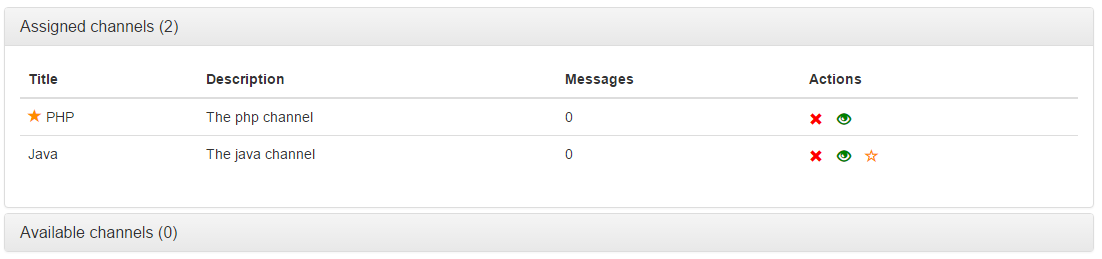
\includegraphics[scale=0.5]{images/start_channels_assigned_after_creation.PNG}
	\caption
	{Implizite Zuweisung}
\end{figure}\\\\
\newpage

\subsubsection{Channels}
Folgend sind die Tests für die Startseite (Channels) angeführt, die nur eingeloggte Benutzer sehen können.\\\\
Folgender Test zeigt die Fehlermeldung wenn versucht wird eine Aktion auszuführen aber der Channel nicht mehr existiert.\\
\begin{figure}[h]
	\centering
	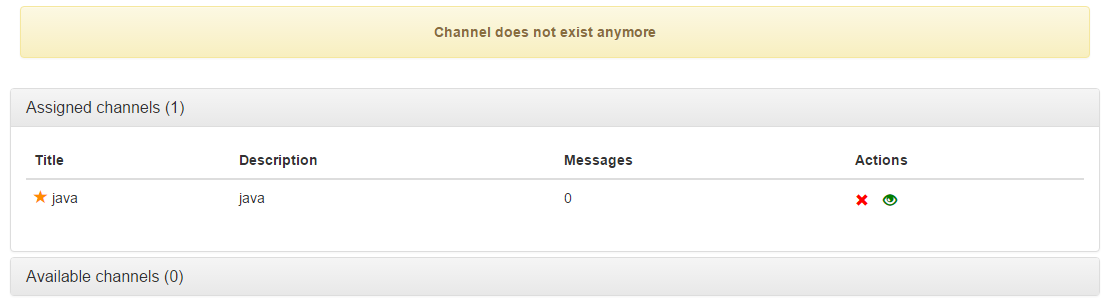
\includegraphics[scale=0.5]{images/start_channels_action_fail.PNG}
	\caption
	{Channel anlegen wenn keine vorhanden}
\end{figure}\\\\

Im Falle das überhaupt kein Channel mehr existiert wird auf die Seite für das Erstellen eines Channels gewechselt, die wiederum solange angezeigt wird bis es mindestens einen Channel gibt.
\newpage

\subsubsection{Channel Chat}
Folgend sind die Tests für die Startseite (Channel Chat) angeführt, die nur eingeloggte Benutzer sehen können.\\\\
Folgender Test zeigt dass bei jeder Aktion die ausgeführt und es den channel nicht mehr gibt die folgende Fehlermeldung ausgegeben wird und der Benutzer auf die Channels Seite weitergeleitet wird, wobei auch hier eine Prüfung erfolgt ob es überhaupt noch Channels gibt. Wenn nicht wird der Benutzer von der Channels Seite auf die Seite New Channel erneut weitergeleitet.
\begin{figure}[h]
	\centering
	
\includegraphics[scale=0.5]{images/start_channel_chat_no_channel_on_action.PNG}
	\caption
	{Kein Channel mehr vorhanden bei Aktionen im Chat}
\end{figure}\\\\

Folgender Test zeigt dass wenn versucht wird eine Nachricht zu editieren es aber diese nicht mehr gibt oder bereits folgende Nachrichten existieren, eine entsprechende Fehlermeldung ausgeben wird.
\begin{figure}[h]
	\centering
	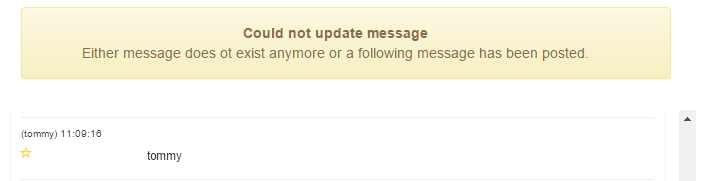
\includegraphics[scale=0.5]{images/start_channel_chat_no_message_or_following.PNG}
	\caption
	{Nachricht nicht mehr vorhanden oder folgende existieren bereits}
\end{figure}\\\\

Folgender Test zeigt dass wenn versucht wird eine Nachricht zu löschen und es bereits folgende Nachrichten gibt oder die Nachricht gelöscht wurde, dass eine entsprechende Fehlermeldung ausgeben wird.
\begin{figure}[h]
	\centering
	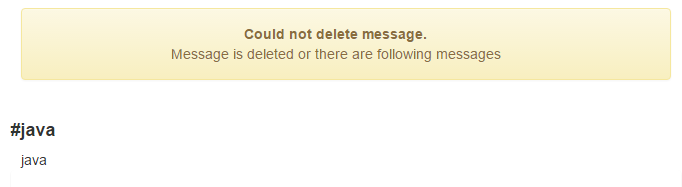
\includegraphics[scale=0.5]{images/start_channel_chat_delete_following_messages.PNG}
	\caption
	{Löschen fehlgeschlagen}
\end{figure}\\\\
\newpage

Folgender Test zeigt dass wenn versucht wird eine Nachricht als Favorit zu setzen aber die Nachricht bereits gelöscht wurde, dass eine entsprechende Fehlermeldung ausgeben wird.
\begin{figure}[h]
	\centering
	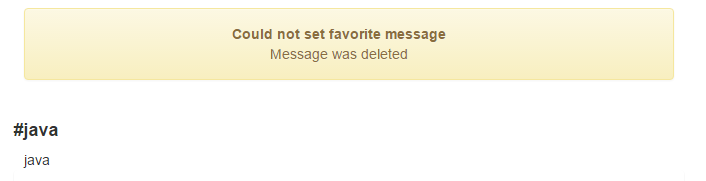
\includegraphics[scale=0.5]{images/start_channel_chat_set_favorite_fail.PNG}
	\caption
	{Löschen fehlgeschlagen}
\end{figure}\\\\

Folgender Test zeigt dass neue Nachrichten beim erstmaligen Anzeigen mit einem Flag gekennzeichnet werden.
\begin{figure}[h]
	\centering
	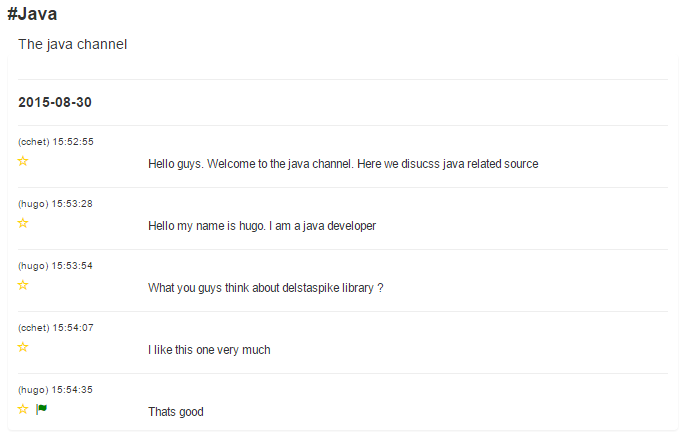
\includegraphics[scale=0.5]{images/start_channel_chat_marked_unread.PNG}
	\caption
	{Markierte ungelesene neue Nachrichten}
\end{figure}\\\\
\newpage

Folgender Test zeigt dass nach alle/Favoriten gefiltert werden kann.\\
Werden nur die Favoriten angezeigt ist ein Bearbeiten ausgeschlossen.\\
Das Menu zeigt hierbei entweder die Option 'Alle' (nur Favoriten) oder 'Favoriten' (Alle) an je nachdem welcher Filter gerade aktiv ist.
\begin{figure}[h]
	\centering
	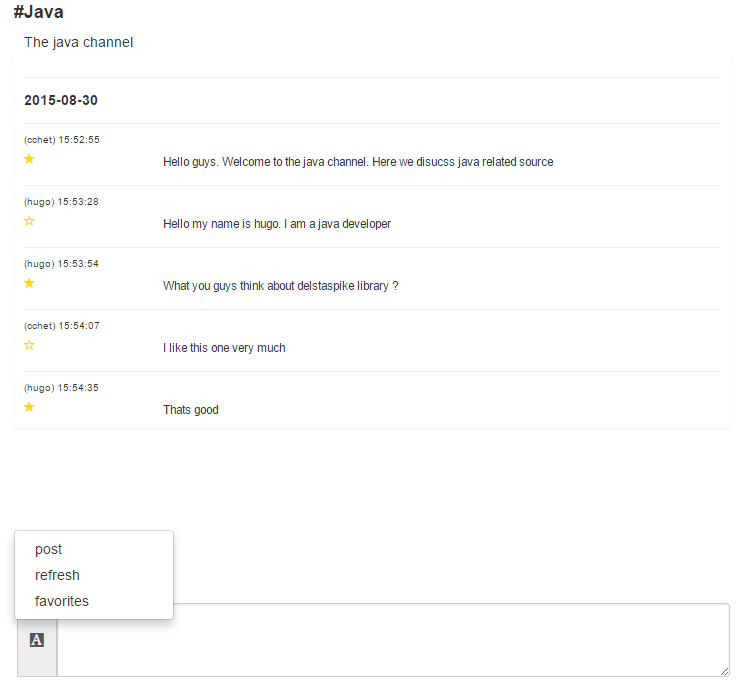
\includegraphics[scale=0.4]{images/start_channel_chat_all.PNG}
	\caption
	{Filter Alle}
\end{figure}\\\\
\begin{figure}[h]
	\centering
	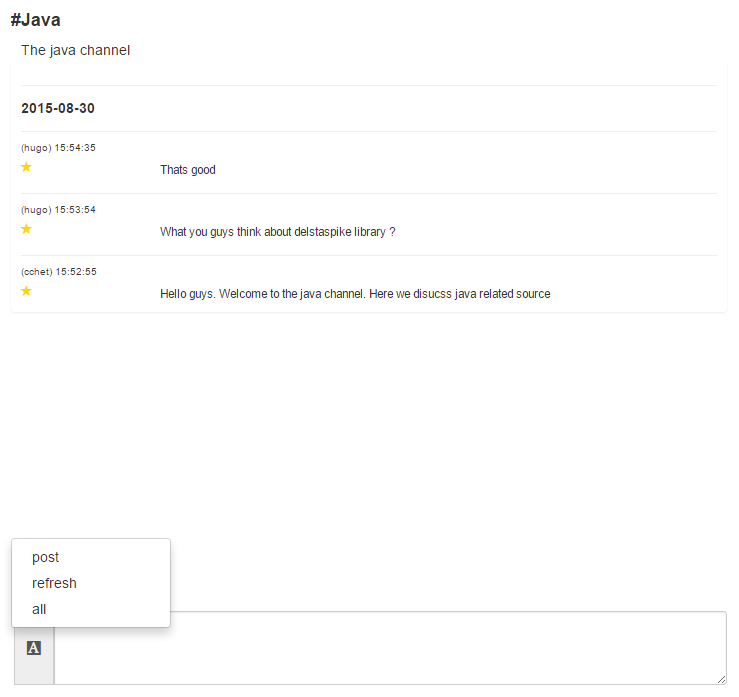
\includegraphics[scale=0.4]{images/start_channel_chat_favorites_only.PNG}
	\caption
	{Filter Favoriten}
\end{figure}\\\\
\newpage



\end{document}  